\documentclass{article}
\usepackage[english,russian]{babel}
\usepackage{amsmath}
\usepackage{amsfonts}
\usepackage{amssymb}
\usepackage{geometry}
\geometry{a4paper, portrait, margin=1in}
\usepackage{hyperref}
\usepackage{esvect}
\usepackage{setspace}
\usepackage{hyperref}
\usepackage{graphicx}

\begin{document}
    \onehalfspacing
    
    \section*{Формулировка задачи}
    Пусть два массивных тела массами $M_1$ и $M_2$ на расстояние $L$ друг от друга вращаются вокруг их общего центра масс по круговым орбитам с угловой скоростью $\omega$.
    Выберем в конкретный момент времени систему отсчета с началом отсчета в их центре масс, ось $x$ напривам от тела массой $M_1$ к телу  массой $M_2$,
    ось $y$ направим перпендикулярно оси $x$. Тела в этой системе отсчета имеют координаты $-r_1$ и $r_2$ соответственно:
    \[ r_1 + r_2 = L \]
    \[ M_1 r_1 = M_2 r_2 \]
    Тогда в этой система отсчета найдется пять так называемых точек Лагранжа, в которых третье тело с массой $m: m \ll M_1, m \ll M_2$
    будет оставаться неподвижным во вращающейся системе отсчёта, связанной с массивными телами. То есть гравитационные силы $\vv{F_1}$ и $\vv{F_2}$,
    действующие на тело с массой $m$ будут равны центробежной, необходимой для движения по окружности с угловой скоростью $\omega$.
    
    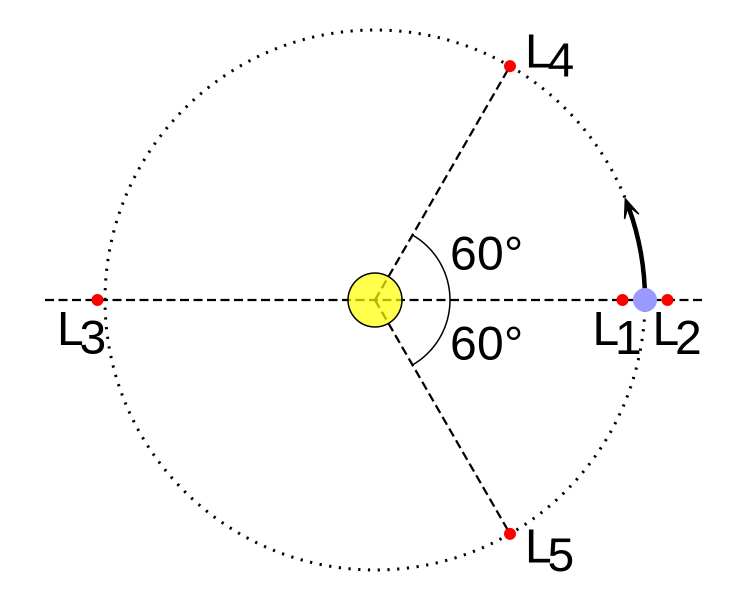
\includegraphics[scale=0.5]{Lagrange_very_massive.png}
    
    \section*{Решение задачи}
    Поместим в такую точку тело массой $m$. Запишем для нее второй закон Ньютона:
    \[ \vv{d_1} = \begin{bmatrix} -r_1 - x \\ - y \end{bmatrix} \]
    \[ \vv{d_2} = \begin{bmatrix} r_2 - x \\ - y \end{bmatrix} \]
    \[ \vv{F_1} = \frac{mM_1G}{d_1^3} \vv{d_1} \]
    \[ \vv{F_2} = \frac{mM_2G}{d_2^3} \vv{d_2} \]
    \[ \vv{F_r} = - m \omega^2 r \hat{{\vv{r}}} = - m \omega^2 \vv{r} \]
    \[ \vv{F_r} = \vv{F_1} + \vv{F_2}  \]
    Перепишем для каждой оси поотдельности:
    \[ - m \omega^2 x =
       \frac{mM_1G}{d_1^3} (-r_1 - x) + \frac{mM_2G}{d_2^3} (r_2 - x) \]
    
    \[ - m \omega^2 y =
       -\frac{mM_1G}{d_1^3} y - \frac{mM_2G}{d_2^3} y \]
    Рассмотрим случай, когда $y \ne 0$, то есть для треугольных точек Лагранжа $L_4$ и $L_5$:
    \[ m \omega^2 =
       \frac{mM_1G}{d_1^3} + \frac{mM_2G}{d_2^3} \]
    \[ - \left( \frac{mM_1G}{d_1^3} + \frac{mM_2G}{d_2^3} \right) x =
       \frac{mM_1G}{d_1^3} (-r_1 - x) + \frac{mM_2G}{d_2^3} (r_2 - x) \]
    \[ \frac{M_1 r_1}{d_1^3} = \frac{M_2 r_2}{d_2^3} \]
    \[ d_1 = d_2 \]
    \[ (r_1 + x)^2 + y^2 = (r_2 - x)^2 + y^2\]
    \[ |r_1 + x| = |r_2 - x| \]
    \[ x = \frac{r_2 - r_1}{2} \]
    \[ d_1 = d_2 = d = \sqrt{ \left(r_2 - \frac{r_2 - r_1}{2}\right)^2 + y^2} = \sqrt{ \left(\frac{L}{2}\right)^2 + y^2 }\]  
    \[ \omega^2 = \frac{(M_1 + M_2)G}{d^3} \]
    Так как вращение происходит с постоянной угловой скоростью:
    \[ M_1 \omega^2 r_1 = \frac{M_1M_2G}{L^2} \]
    \[ M_2 \omega^2 r_2 = \frac{M_1M_2G}{L^2} \]
    \[ \omega^2 (r_1 + r_2) = \frac{\left(M_1 + M_2\right)G}{L^2} \]
    \[ \omega^2 = \frac{(M_1 + M_2)G}{L^3} \]
    \[ d = L \]
    \[ \left(\frac{L}{2}\right)^2 + y^2 = L^2 \]
    \[ y = \pm \frac{\sqrt{3}}{2}L \]
    То есть точки $L_4$ и $L_5$ находятся в третьих вершинах равносторонних треугольников, построенных на соединящем тела массами $M_1$ и $M_2$ отрезке.
    \\
    Теперь рассмотрим случай, когда $y = 0$ для так называемых коллинеарных точек Лагранжа $L_1$, $L_2$ и $L_3$:
    \[ m \omega^2 x = \frac{ m\left( M_1 + M_2 \right)G }{L^3} x =
       \frac{M_1}{|r_1 + x|^3} (r_1 + x) + \frac{M_2}{|x - r_2|^3} (x - r_2) \]
    Такое уравнение можно решить только численными методами, или если сделать предположение, что $M_1 \gg M_2$ (как например в система Солнце-Земля
    или Земля-Луна).
    \\
    Рассмотрим каждый из четырех вариантов расскрытия модуля.
    \\
    Первый случай, когда малое тело слева от обоих больших тел (точка $L_3$):
    \[ |r_1 + x| < 0 \land |x - r_2| < 0 \]
    \[ \frac{\left( M_1 + M_2 \right) }{L^3} x =
       -\frac{M_1}{(r_1 + x)^2} - \frac{M_2}{(x - r_2)^2} \]
    \[ \frac{\left( M_1 + M_2 \right) }{L^3} x (r_1 + x)^2 (x - r_2)^2 =
       - M_1 (x - r_2)^2 - M_2 (r_1 + x)^2 \]
    \[ \frac{x(r_1 + x)^2}{L^3} = -1 \]
    \[ x \approx -L \]
    Второй и третий случай, когда малое тело находится справа от тела массой $M_1$ и поочередно слева и справа от тела массой $M_2$ (точки $L_1$ и $L_2$).
    Решение будем искать в виде $x = L \mp l$:
    \[ |r_1 + x| > 0 \land |x - r_2| < 0 \]
    \[ \frac{\left( M_1 + M_2 \right) }{L^3} (L - l) =
       \frac{M_1}{(r_1 + L - l)^2} - \frac{M_2}{l^2} \]
    \[ |r_1 + x| > 0 \land |x - r_2| > 0 \]
    \[ \frac{\left( M_1 + M_2 \right) }{L^3} (L + l) =
       \frac{M_1}{(r_1 + L + l)^2} + \frac{M_2}{l^2} \]
    \[ \frac{2 \left( M_1 + M_2 \right) l}{L^3} = \frac{2M_2}{l^2} + \frac{M_1}{(r_1 + L + l)^2} - \frac{M_1}{(r_1 + L - l)^2} \]
    \[ \frac{M_1 l}{L^3} = \frac{M_2}{l^2} + \frac{M_1}{2(L + l)^2} - \frac{M_1}{2(L - l)^2} \]
    \[ \frac{M_1 l}{L^3} = \frac{M_2}{l^2} - \frac{2 M_1 l}{L^3} \]
    \[ \frac{3 M_1 l}{L^3} = \frac{M_2}{l^2} \]
    \[ l^3 = \frac{M_2}{3 M_1} L^3 \]
    \[ l = \sqrt[3]{\frac{M_2}{3 M_1}} L \]
    Расскрытие $|r_1 + x| < 0 \land |x - r_2| > 0$ не имеет смысла, так как в таком случае малое тело левее левого тела, но правее правого.

    \section*{Практическое применение решения задачи}
    В точках $L_4$ и $L_5$ малое тело находится в устойчивом равновесии при условие, что отношение масс больших тел не менее $25$.
    Тогда при малом отклонении оно будет вращаться вокруг них. В точках $L_1$, $L_2$ и $L_3$ равновесие неустойчивое.
    В системе Солнце-Земля, в точке $L_1$ размещаются космической обсерватории для наблюдения Солнца, в точке $L_2$ в $2021$ будет размещен телескоп "Джеймс Уэбб".
    \\
    В системе Земля-Луна, точка $L_1$ могла бы использовать для заправочной станции, точка $L_2$ -- для спутниковой связи с обратной стороной Луны.
    \\
    В точках $L_4$ и $L_5$ обычно скапливаются астероиды.
    
    \section*{Источники}
    \url{https://ru.wikipedia.org/wiki/%D0%A2%D0%BE%D1%87%D0%BA%D0%B8_%D0%9B%D0%B0%D0%B3%D1%80%D0%B0%D0%BD%D0%B6%D0%B0}
    \\
    \url{https://en.wikipedia.org/wiki/Lagrange_point}
    \\
    \url{https://solarsystem.nasa.gov/resources/754/what-is-a-lagrange-point}
    \\
    \url{https://www.youtube.com/playlist?list=PLbfY1f0QFa4OmdgNEP_vESH6w31aFJS5y}
    \\

\end{document}
